% TikZ schematic: Image Formation + Enhancement Pipeline (standalone compile)
\documentclass[tikz,border=10pt]{standalone}
\usepackage{tikz}
\usetikzlibrary{positioning,arrows.meta,decorations.pathreplacing,calc}

\begin{document}
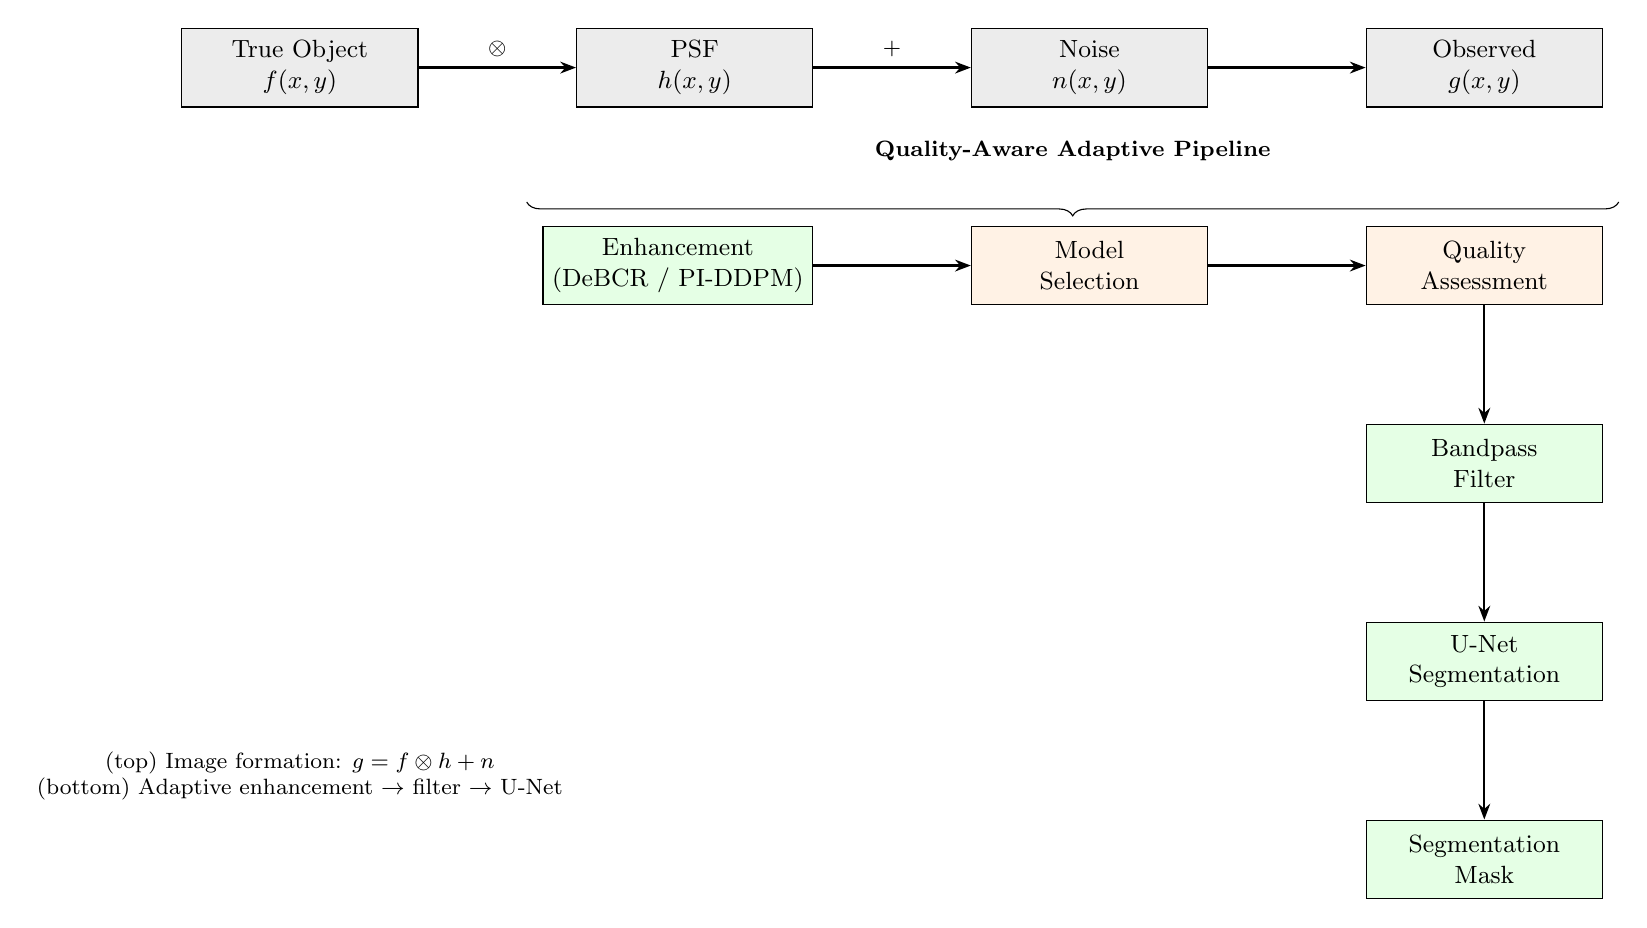
\begin{tikzpicture}[
    node distance=1.5cm and 2cm,
    block/.style={rectangle, draw, fill=blue!8, minimum width=3cm, minimum height=1cm, align=center, font=\small},
    arrow/.style={-{Stealth[length=2mm]}, thick},
    label/.style={font=\footnotesize}
]

% Image formation
\node[block, fill=gray!15] (obj) {True Object\\$f(x,y)$};
\node[block, fill=gray!15, right=of obj] (psf) {PSF\\$h(x,y)$};
\node[block, fill=gray!15, right=of psf] (noise) {Noise\\$n(x,y)$};
\node[block, fill=gray!15, right=of noise] (obs) {Observed\\$g(x,y)$};

\draw[arrow] (obj) -- node[above, label] {$\otimes$} (psf);
\draw[arrow] (psf) -- node[above, label] {$+$} (noise);
\draw[arrow] (noise) -- (obs);

% Enhancement pipeline (below)
\node[block, fill=orange!10, below=1.5cm of obs] (assess) {Quality\\Assessment};
\node[block, fill=orange!10, left=of assess] (select) {Model\\Selection};
\node[block, fill=green!10, left=of select] (enhance) {Enhancement\\(DeBCR / PI-DDPM)};
\node[block, fill=green!10, below=of assess] (filt) {Bandpass\\Filter};
\node[block, fill=green!10, below=of filt] (seg) {U-Net\\Segmentation};
\node[block, fill=green!10, below=of seg] (out) {Segmentation\\Mask};

\draw[arrow] (enhance) -- (select);
\draw[arrow] (select) -- (assess);
\draw[arrow] (assess) -- (filt);
\draw[arrow] (filt) -- (seg);
\draw[arrow] (seg) -- (out);

% Brace label
\draw[decorate, decoration={brace, amplitude=5pt, mirror}]
    ($(enhance.north west)+(-0.2,0.3)$) -- ($(assess.north east)+(0.2,0.3)$)
    node[midway, above=0.4cm, label] {\textbf{Quality-Aware Adaptive Pipeline}};

% Caption note
\node[font=\footnotesize, align=center] at (0,-9) {(top) Image formation: $g = f \otimes h + n$ \\ (bottom) Adaptive enhancement $\rightarrow$ filter $\rightarrow$ U-Net};

\end{tikzpicture}
\end{document}
